\section{Struktur}

Dette pattern består af 2 vitale dele, Read siden og Write siden, Disse 2 dele, gør at patternet kan effektivt skrive eller læse til en data store. Princippet er at disse delen er Ren (Pure) og altså kun gør det som den er sat til. Write siden skriver kun til Datastore og returnere ikke nogen form for tilstand tilbage. Read siden mutere ikke data, men returnere kun Data. Disse handlinger er gjort igennem Commands og Queries, som lige præcis gør dette. 

\subsection{Generelt}

\begin{figure}[H]
	\center
	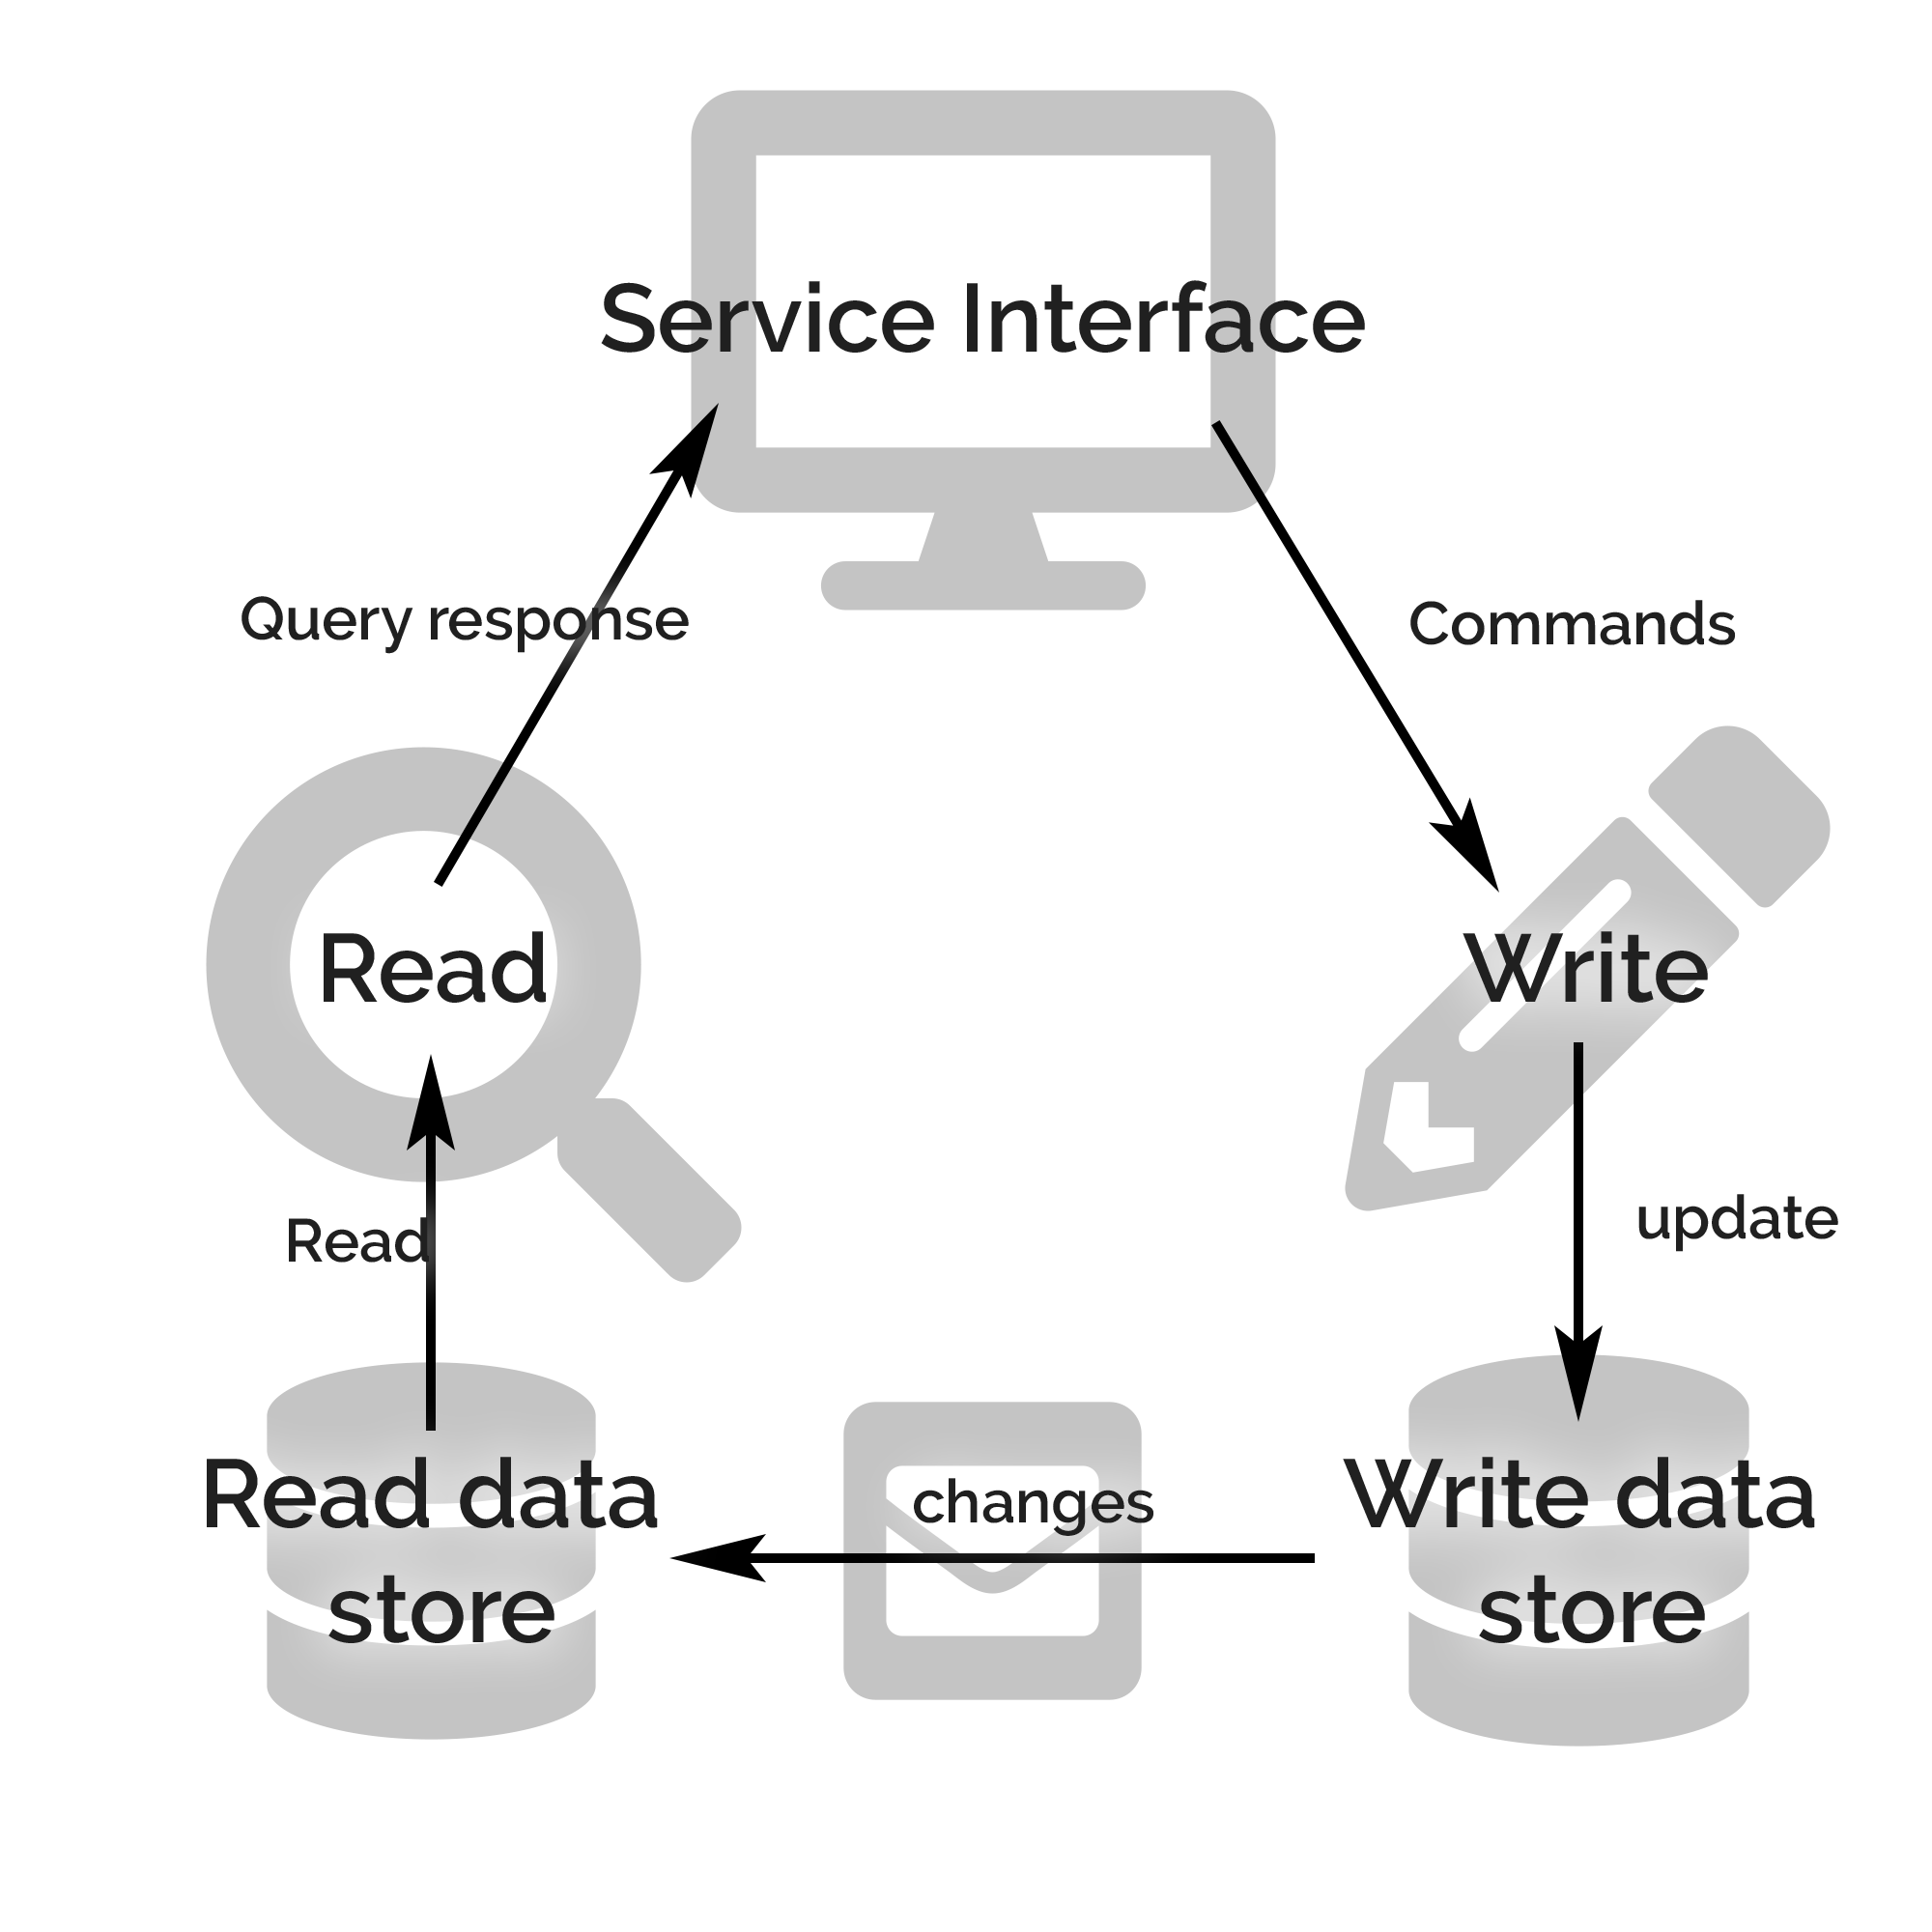
\includegraphics[width=0.7\textwidth]{CQRS-Model.png}
	\caption{Simpel CQRS med Read og Write}
	\label{fig:cqrs-model}
\end{figure}

\subsection{Read}


\subsection{Write}

